\documentclass[../thesis.tex]{subfiles}

\begin{document}

\chapter{Data Analysis of Patient Admissions into ABUHB}\label{chp:Data}

\section{Introduction}
This section aims to provide an overview of data received from the Aneurin Bevan University Health Board (ABUHB), to gain a deeper understanding into the current practice and trends within ABUHB.

Within this research, three years worth of data has been used from April 2017 to March 2020 with two data sets being amalgamated. 


The first data set, discussed in Section \ref{Sec:Admission}, is from Myrddin, the patient administration system (PAS). Myrddin stores all patient contact details, outpatient appointments, generates letters for patients, and specifically for this research, inpatient details.

The second data set, discussed in Section \ref{Sec:Radis}, is the Welsh Radiological Information Systems (RadIS). RadIS is the IT system that stores and keep tracks of which patients have received scans. 
%https://senedd.assembly.wales/documents/s73101/PAC5-08-18%20P3%20-%20AGW%20Report%20-%20Informatics%20Systems%20in%20NHS%20Wales.pdf
%The second data set, discussed in Subsection \ref{Sec:Radis}, contains patient scan data for the time period.Welsh Radiology Information System %https://dhcw.nhs.wales/news/archived-news/radis2-completes-national-rollout/


%\subsection{Criteria of Patients} \label{Sec:CritOfPatients}
Prior to any analysis occurring, data cleansing was performed to ensure incorrect and incomplete entries were removed. Additionally, a criteria was set to ensure the patients were relevant to the study. The following criteria was set:
\begin{enumerate}
    \item Only complete patient information files were included i.e., no missing entries. Diagnosis was excluded from this, since patients could be admitted to hospital and discharged with no formal diagnosis.
    \item Patients were only included if they were aged 65 and over \cite{OECD}.
    \item For the RadIS data set, patients were required to be admitted within hospital.
\end{enumerate}


Figure \ref{fig:FlowChartData} provides an overview of the data cleansing process for both data sets. For the admission data set, a total of 165,055 patients were included within the study, of which 15,483 scan records were present from the RadIS data set.


%Each year of data was provided separately, so the first step required all three years to be merged. Firstly, any patients who did not have an NHS number were removed from analysis as their admission or scan could then not be matched with any relevant data, i.e., readmission, scan information or transfer between hospitals. As this work is specifically focusing on the elderly, a base line age of 65 was used for analysis, and those aged under 65 were removed from the data  For the Admission data set, if there was no admission date or discharge date, they were removed from the data. For the Radis data set, if the patient was not an inpatient, they were removed from analysis. This in total resulted in 165,118 patient records for admission data set, and 12,350 for the Radis data set, as seen in Figure \ref{Fig:Flowchart}.

%\begin{figure}[h!]
%\centering
%\begin{tikzpicture}[scale=0.75, transform shape,node distance=3.2cm]
%\node (pro1) [process, right of =pro3] {\parbox{2.5cm}{\centering 2019 - 2020 \\135,513} };%{number1};
%\node (pro2) [process, left of =pro3] {\parbox{2.5cm}{\centering 2017 - 2018 \\131,880} };
%\node (pro3) [process, right of =pro2] {\parbox{2.5cm}{\centering 2018 - 2019 \\138,128} };
%\node (pro4) [process, below of =pro3] {405,521};
%\node (pro5) [process, below of =pro4] {405,128};
%\node (pro6) [process, below of =pro5] {405,055};
%\node (pro7) [process, below of =pro6] {165,055};
%\node (stop1) [startstop, below of =pro6] {\begin{tabular}{c} 165,055 Patients \\ in Admission Data
%\end{tabular}}; 
%\draw [arrow] (pro1) -- (pro4);
%\draw [arrow] (pro2) -- (pro4);
%\draw [arrow] (pro3) -- (pro4);
%\draw [arrow] (pro4) -- node [anchor=west]{\begin{tabular}{c} 393 Removed \\ No NHS Number
%\end{tabular}}  (pro5);
%\draw [arrow] (pro5) -- node [anchor=west]{\begin{tabular}{c} 73 Removed \\ No Admission/Discharge
%\end{tabular}}  (pro6);
%\draw [arrow] (pro6) -- node [anchor=west]{\begin{tabular}{c} 240,000 Removed \\ Under 65
%\end{tabular}}  (stop1);
%\node (pro10) [process, right of =pro1] {\parbox{2.5cm}{\centering 2017 - 2018 \\81,020}};
%\node (pro11) [process, right of =pro10] {\parbox{2.5cm}{\centering 2018 - 2019 \\83,109}};
%\node (pro12) [process, right of =pro11] {\parbox{2.5cm}{\centering 2019 - 2020 \\81,158}};
%\node (pro13) [process, below of =pro11] {245,287};
%%\node (pro15) [process, below of =pro14] {140,509};
%\node (pro16) [process, below of =pro15] {15,483};
%\node (stop2) [startstop, below of =pro15]{\begin{tabular}{c} 15,483 Patients \\ in RadIS Data
%\end{tabular}}; 
%\draw [arrow] (pro10) -- (pro13);
%\draw [arrow] (pro11) -- (pro13);
%\draw [arrow] (pro12) -- (pro13);
%\draw [arrow] (pro13) -- node [anchor=west]{\begin{tabular}{c} 418 Removed \\ No NHS Number
%\end{tabular}}  (pro14);
%\draw [arrow] (pro14) -- node [anchor=west]{\begin{tabular}{c} 104,360 Removed \\ Under 65
%\end{tabular}}  (pro15);
%\draw [arrow] (pro15) -- node [anchor=west]{\begin{tabular}{c}  125,026 Removed \\ Not an inpatient
%\end{tabular}}  (stop2);
%\draw[arrow] (pro15) -- (pro16);
%\draw[arrow] (pro15) -- (stop2);
%\draw[arrow] (pro15) -- node [midway](LtoB){} (stop2);
%\draw[arrow] (stop1) -- node [above,sloped] {} (LtoB);

%\end{tikzpicture}
%\caption{Flow Chart of Data Criteria}
%\label{fig:FlowChartData}
%\end{figure}

\begin{figure}[h!]
\centering
\begin{tikzpicture}[scale=0.75, transform shape,node distance=3.2cm]

\node (pro1) [process, right of =pro3] {\parbox{2.5cm}{\centering 2019 - 2020 \\135,513} };%{number1};
\node (pro2) [process, left of =pro3] {\parbox{2.5cm}{\centering 2017 - 2018 \\131,896} };
\node (pro3) [process, right of =pro2] {\parbox{2.5cm}{\centering 2018 - 2019 \\138,128} };

\node (pro4) [process, below of =pro3] {405,537};

\node (pro5) [process, below of =pro4] {405,144};

\node (pro6) [process, below of =pro5] {405,118};

%\node (pro7) [process, below of =pro6] {165,055};
\node (stop1) [startstop, below of =pro6] {\begin{tabular}{c} 165,118 Patients \\ in Admission Data
\end{tabular}}; 

\draw [arrow] (pro1) -- (pro4);
\draw [arrow] (pro2) -- (pro4);
\draw [arrow] (pro3) -- (pro4);
\draw [arrow] (pro4) -- node [anchor=west]{\begin{tabular}{c} 393 Removed \\ No NHS Number
\end{tabular}}  (pro5);
\draw [arrow] (pro5) -- node [anchor=west]{\begin{tabular}{c} 73 Removed \\ No Admission/Discharge
\end{tabular}}  (pro6);
\draw [arrow] (pro6) -- node [anchor=west]{\begin{tabular}{c} 240,000 Removed \\ Under 65
\end{tabular}}  (stop1);

\node (pro10) [process, right of =pro1] {\parbox{2.5cm}{\centering 2017 - 2018 \\81,020}};
\node (pro11) [process, right of =pro10] {\parbox{2.5cm}{\centering 2018 - 2019 \\83,109}};
\node (pro12) [process, right of =pro11] {\parbox{2.5cm}{\centering 2019 - 2020 \\81,158}};
\node (pro13) [process, below of =pro11] {245,287};
\node (pro14) [process, below of =pro13] {244,869};
\node (pro15) [process, below of =pro14] {140,509};

\node (stop2) [startstop, below of =pro15]{\begin{tabular}{c} 15,483 Patients \\ in RadIS Data
\end{tabular}}; 
\draw [arrow] (pro10) -- (pro13);
\draw [arrow] (pro11) -- (pro13);
\draw [arrow] (pro12) -- (pro13);

\draw [arrow] (pro13) -- node [anchor=west]{\begin{tabular}{c} 418 Removed \\ No NHS Number
\end{tabular}}  (pro14);
\draw [arrow] (pro14) -- node [anchor=west]{\begin{tabular}{c} 104,360 Removed \\ Under 65
\end{tabular}}  (pro15);
\draw [arrow] (pro15) -- node [anchor=west]{\begin{tabular}{c}  125,026 Removed \\ Not an inpatient
\end{tabular}}  (stop2);
\draw[arrow] (pro15) -- node [midway](LtoB){} (stop2);
\draw[arrow] (stop1) -- node [above,sloped] {} (LtoB);
\end{tikzpicture}
\caption{Flow Chart of Data Criteria}
\label{fig:FlowChartData}
\end{figure}

\section{Admission Data Set}\label{Sec:Admission}
This section discusses the 165,188 patients that were admitted into hospital between April 2017 and March 2020.
\begin{figure}[h!]
    \centering
    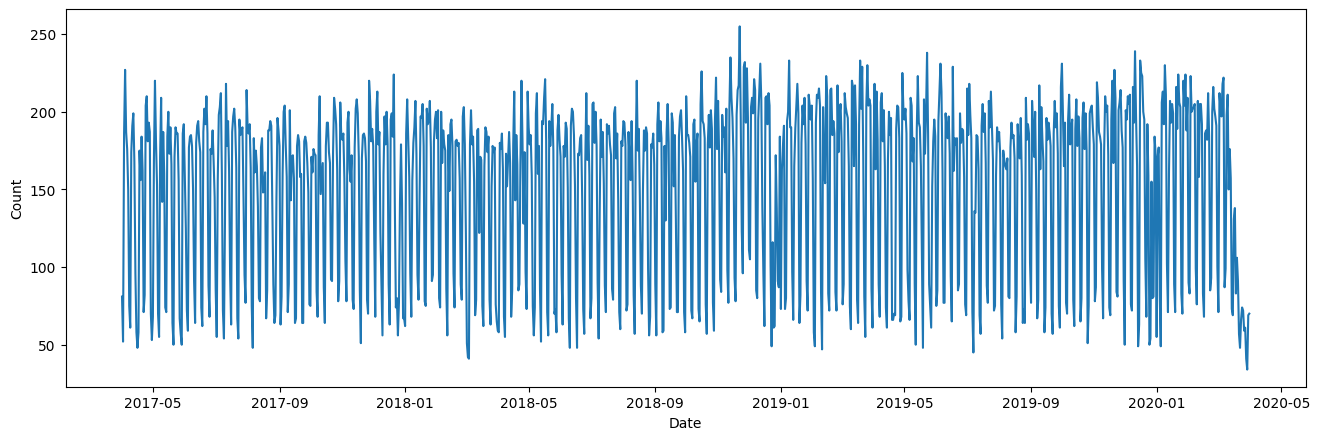
\includegraphics[width=\textwidth]{Chapters/Chapter3/Figures/Admission per day.png}
    \caption{Daily Count of Admissions into ABUHB}
    \label{fig:AdmissionCount}
\end{figure}

Figure \ref{fig:AdmissionCount} displays the daily count of admissions into ABHUB over time. The fluctuations within the data suggest seasonality is present as often found within healthcare data \cite{Upshur2005}.
Analysing by a year to year basis, (running April to March), the the number of patients remains fairly consistent over the three years:
\begin{itemize}
    \item 2017-2018: 53,256 (32.25\%)
    \item 2018-2019: 56,050 (33.95\%)
    \item 2019-2022: 55,812 (33.80\%)
\end{itemize}
Breaking this down further, it can be seen within Figure \ref{fig:AdmissionCountyear}, that there is little variation between the trends each year.
\begin{figure}[h!]
    \centering
    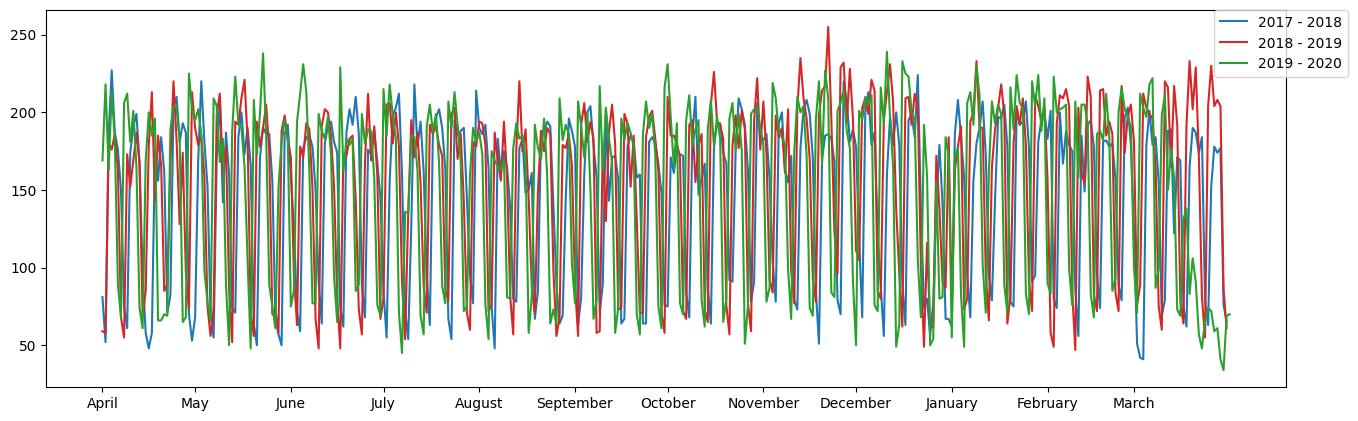
\includegraphics[width=\textwidth]{Chapters/Chapter3/Figures/Admission each year.png}
    \caption{Daily Count of Admissions into ABUHB split by year}
    \label{fig:AdmissionCountyear}
\end{figure}

Data from April 2020, was not included within the study due to the COVID-19 pandemic, and the skewed effects this would have had on admission data \cite{Venkatesan2020}. The effect of COVID-19 can be seen from March 2020, where admissions for patients aged 65 and older had began to decrease.

Within the data set, there were 16 different attributes relating to a patients admission and discharge, with a detailed overview provided in Table \ref{tab:AttributesAdmission}

%\begin{landscape}
\begin{longtable}{p{3cm}lp{5cm}ccc}
\toprule
{ \textbf{Attribute}} & {\textbf{Data type}} & {\textbf{Distinct attribute values}} & \multicolumn{2}{c}{ \textbf{Documentation}}
\tabularnewline
& &\textbf{or bins} & {at admission }&  { Tdischarge}\tabularnewline
\midrule
\endhead

{Admission Date} & {Continuous} & {1096 (e.g. 20170401)}&\checkmark & \tabularnewline\midrule
{Admission Method} & {Nominal} &  {17 (e.g. Elective waiting list)} &\checkmark & \tabularnewline\midrule
{Admission Source} & {Nominal} & {26 (e.g. Usual place of residence)}&\checkmark & \tabularnewline\midrule
{Admission Time} & {Continuous} & {1440 (hh:mm)}&\checkmark & \tabularnewline\midrule
{Date of Birth} & {Continuous} & {12038 (e.g. 20000101)} &\checkmark & \tabularnewline\midrule
{Diagnosis} & {Nominal} &{2758 (e.g. Fracture of neck of femur, Congestive heart failure)} &\checkmark & \tabularnewline\midrule
{Discharge Date} &{Continuous} & {1167 (e.g. 20170401)}& &\checkmark  \tabularnewline\midrule
{Discharge Destination} &{Nominal} &{26 (e.g. Death, Own home, Patient transfer within same health board/trust)}  &&\checkmark \tabularnewline\midrule
{Discharge Time} &{Continuous} & {1440 (hh:mm)} &&\checkmark \tabularnewline\midrule
{Hospital} & {Nominal} & {14 (e.g. Chepstow Community Hospital)} &\checkmark & \tabularnewline\midrule
{NHS Number} & {Nominal} & {66,289} &\checkmark & \tabularnewline\midrule
{Patient Borough} & {Nominal} & {174 (e.g. Newport LHB, Monmouthshire LHB)} &\checkmark & \tabularnewline\midrule 
{Patient Postcode} & {Nominal} &{13819 (e.g. NP20 2UB)} &\checkmark & \tabularnewline\midrule
{Registered GP} & {Nominal} & {1313 (e.g. G7600177)}&\checkmark & \tabularnewline\midrule 
{Registered GP practice code} & {Nominal} & {618 (e.g. W93007)} &\checkmark & \tabularnewline\midrule 
{Specialty} & {Nominal} & {29 (e.g. Care of the Elderly, Neurology)}&\checkmark & \tabularnewline\midrule
\bottomrule
\caption{List of attributes within Admission data set\label{tab:AttributesAdmission}}
\end{longtable}
%\end{landscape}

There are 66,289 unique NHS numbers, meaning 98,829 stays are either part of a care spell or a separate admission. The data did not give any indication regarding patient care spells, i.e., where they had been transferred between hospitals. Therefore, it was decided that if a patient had been discharged and readmitted on the same day, then this would fall into the `care spell’ category. In total there were 9,464 care spell episodes. This can be broken down further into the number of transfers (Table \ref{Tab:Spell}).
\begin{table}[H]
    \centering
    \begin{tabular}{cccccccc}\toprule
    \textbf{No. of Transfers} & \textbf{1} & \textbf{2} & \textbf{3} & \textbf{4} & \textbf{5} & \textbf{6} & \textbf{7}   \\ \midrule
\textbf{Total} & 8435 & 313 & 50 & 22 & 4 & 1& 1\\ \bottomrule
    \end{tabular}
    \caption{Number of Patient Transfers}
    \label{Tab:Spell}
\end{table}
The patient who was transferred/readmitted seven times had a total length of stay of 219 days, primarily moving between Royal Gwent Hospital and County Hospital before being discharged to a non-NHS care home.

\subsection{Patient Demographic Attributes}
\subsubsection{Hospital Admittance}
As discussed in Section \ref{sec:ABUHB}, there were fourteen hospital locations used within this research.
The majority of admissions (49.41\%) were located at Royal Gwent Hospital (RGH). Further expanding this, 93.41\% of patients are accounted for in the top four hospitals: Royal Gwent Hospital (RGH), Nevill Hall Hospital (NHH) (26.50\%), Ysbyty Ystrad Fawr (YYF) (11.29\%) and St. Woolos Hospital (6.21\%).

\hl{Figure of hospital admissions here - potentially split by year}
\begin{figure}[H]
    \centering
 %   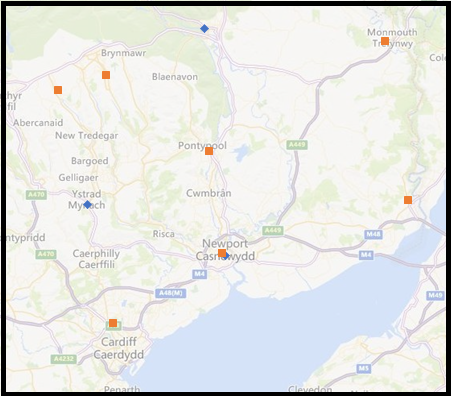
\includegraphics[width = 8cm]{Chapter3/Figures/SE Wales.png}
    \caption{Graph of Hospital Admissions} %\hl{Can look at improving map}}
    \label{Fig:Hospital}
\end{figure}

Using patient postcodes, we are able to determine the distance between the hospital attended and their residing location.

The first method to achieve this was using the Haversine formula, which calculates `as the grow flies' distance between two points, and therefore the shortest distance between the two.
Equations \ref{eq:Haversine1} - \ref{eq:Haversine3} display the Haversine formula.
\begin{align}\label{eq:Haversine1}
    a&= \sin^{2}(\Delta\Phi/2) +\cos\Phi_{1}\cos\Phi_{2}\sin^{2}(\Delta\lambda/2)\\
    c &= 2* \atantwo(\sqrt{a},\sqrt{(1-a)}\label{eq:Haversine2}\\
    d &= R * c\label{eq:Haversine3}
\end{align}
where $\Phi$ is latitude, $\lambda$ is longitude and $R$ is the earths radius.%6371km

Figure \ref{fig:distance} displays the results of how many patient attend their local hospital using the Haversine formula. The results show that in 28.84\% of cases, most patients attend their closest hospital.
\begin{figure}[h!]
    \centering
    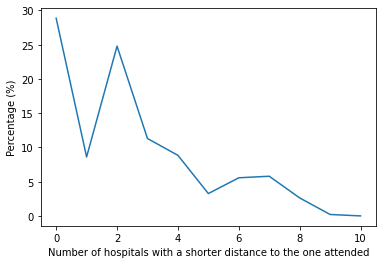
\includegraphics[width = 8cm]{Chapters/Chapter3/Figures/DistanceHospital.png}
    \caption{Proportion of patients against nearest hospital attended}
    \label{fig:distance}
\end{figure}

The second method to achieve distance between patient postcode and hospital attended is the `by road' method. This is achieved by using Google API's to link to a mapping database. 
\hl{Discuss how these distances were calculated and discuss if/what the differences are.}

\subsubsection{Patient Borough}
The borough a patient was admitted from provides a wide scale look at where patients are arriving from, compared to analysing the patient postcodes. ABUHB covers six regions in Wales: Blaenau Gwent, Caerphilly, Monmouthshire, Newport, Torfaen and South Powys. These six regions account for 98.29\% of admissions (Table \ref{Tab:Locations}).

\begin{table}[H]
    \centering\scalebox{0.8}{
    \begin{tabular}{lcccccc}\toprule
    \textbf{Region} &Caerphilly &Newport &Torfaen & Monmouthshire & Blaenau Gwent & Powys \\ \midrule
\textbf{Percentage}& 23.74\% & 23.51\% &  17.12\% & 16.84\% & 16.84\% & 3.81\%\\
 \bottomrule
    \end{tabular}}
    \caption{ABUHB Admission Locations}
    \label{Tab:Locations}
\end{table}

However, in total there are 173 boroughs from which patients arrive from. Figure \ref{Fig:Heatmap} shows the density of patient postcodes for admissions throughout the UK. As expected, a high proportion live in the ABUHB area, with a higher density of arrivals from more populous areas such as Newport and Caerphilly (Figure \ref{Fig:Heatmap2}). However, Figure \ref{Fig:Heatmap1} shows some clusters of admissions from other areas in South Wales such as Swansea, to further afield in places in England including London.

\begin{figure}
\centering
\begin{subfigure}{.5\textwidth}
  \centering
  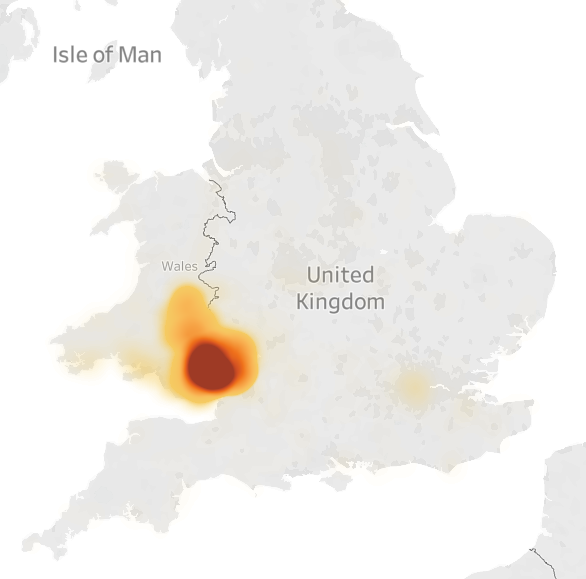
\includegraphics[scale=0.5]{Chapters/Chapter3/Figures/UK-tab.png}
  \caption{UK Wide}
  \label{Fig:Heatmap1}
\end{subfigure}%
\begin{subfigure}{.5\textwidth}
  \centering
  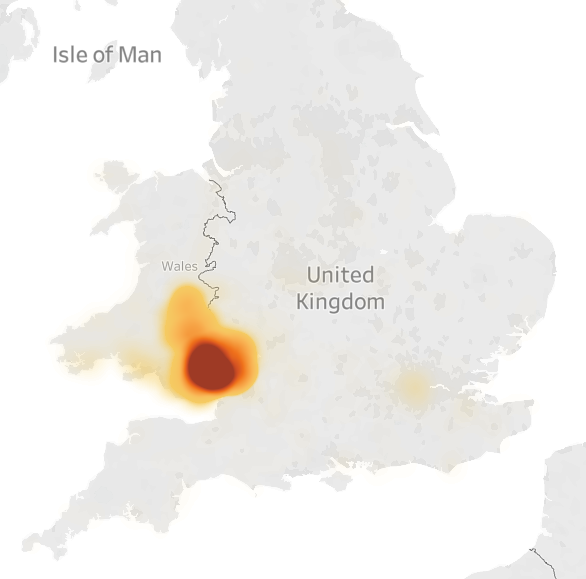
\includegraphics[scale=0.45]{Chapters/Chapter3/Figures/UK-tab.png}
  \caption{Wales focused}
  \label{Fig:Heatmap2}
\end{subfigure}
\caption{Heat Map of Patient Postcodes \hl{Look at producing more informative graphs}}
\label{Fig:Heatmap}
\end{figure}


\subsection{Patient Clinical Attributes}
\subsubsection{Age of Patients}
The age of patients had a lower bound of 65, with the oldest age of 107 years old. Figure \ref{Fig:Age} illustrates that the number of patients increase from age 65 to 71, with the count decreasing for those aged 78 and older. The mean age was 77 years with a standard deviation of eight years.

\begin{figure}[H]
    \centering
    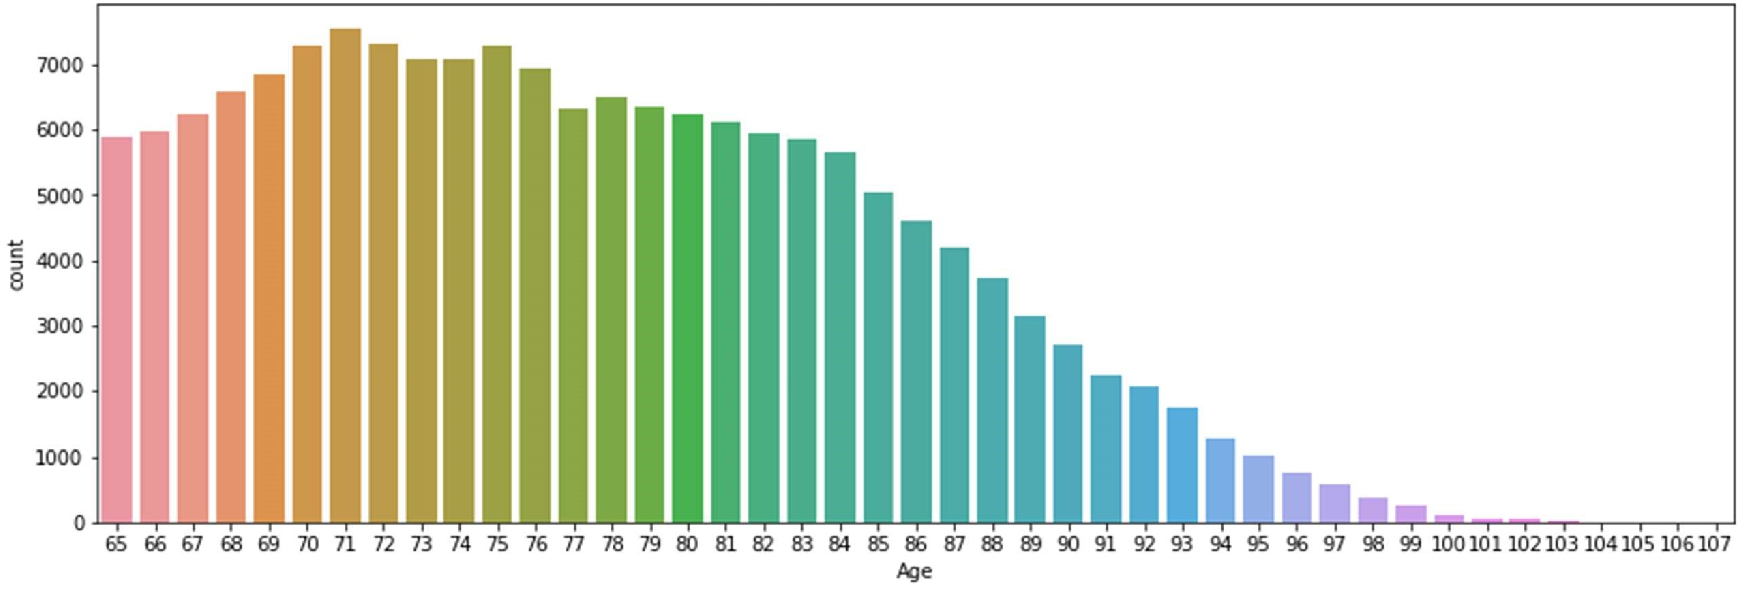
\includegraphics[width=\textwidth]{Chapter3/Figures/Age.pdf}
    \caption{Nominal Age of Patients}
    \label{Fig:Age}
\end{figure}
Due to the large range of ages, these can be grouped into 5-year age groups (Figure \ref{Fig:AgeGroup}). Patients who are aged 95 and older have been grouped into the 95+ age group due to the small quantity of patients. The highest frequency group is 70-74 with 22.02\% of patients being in this age group.
\begin{figure}[H]
    \centering
    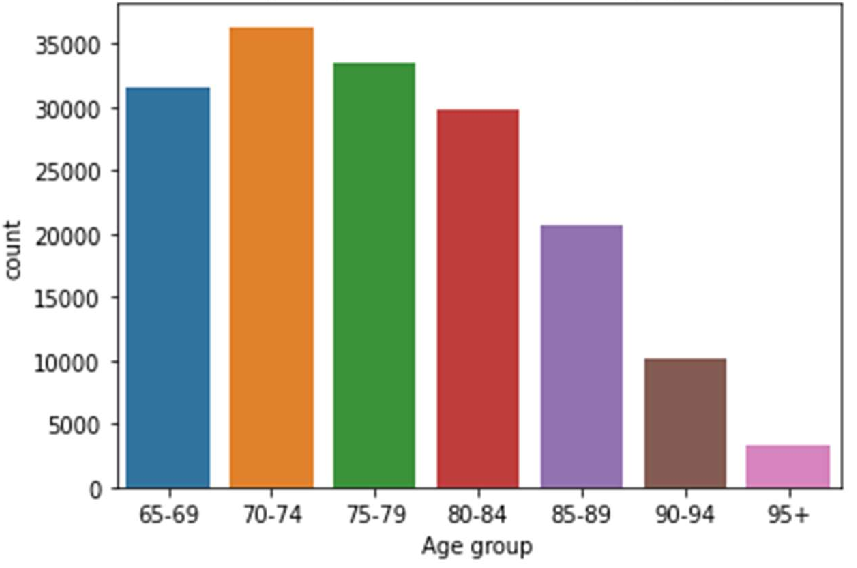
\includegraphics[width = 8cm]{Chapter3/Figures/Age group.pdf}
    \caption{Categorical Age of Patients}
    \label{Fig:AgeGroup}
\end{figure}

\subsubsection{Day of Admission} 
Figure \ref{Fig:AdmissionDay} shows the highest frequency of admissions occur on a Tuesday (18.04\%), following by Thursdays (17.84\%). Patients who are admitted over a weekend account for 14.08\% of total admissions.
\begin{figure}[H]
    \centering
    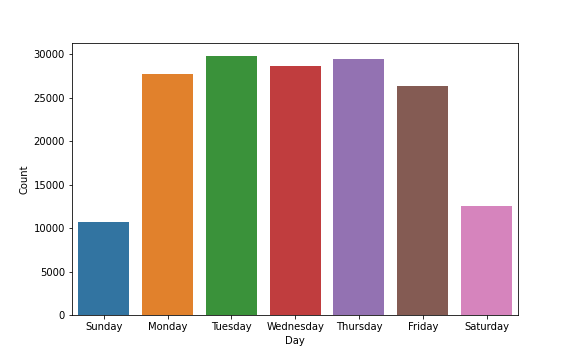
\includegraphics[width = 9.5cm]{Chapter3/Figures/Day.png}
    \caption{Admissions by Day}
    \label{Fig:AdmissionDay}
\end{figure}
Splitting the admissions into hourly arrivals, those patients admitted on a weekday peaked  between 7am and 10am, with a secondary peak between 12pm and 1pm (Figure \ref{Fig:AdmissionTimes}). Weekend admissions are fairly consistent across all hours with a peak between 7am and 9am, and then 12pm and 1pm. Across all days, admissions between 9pm and 7am were low.
\begin{figure}[H]
    \centering
    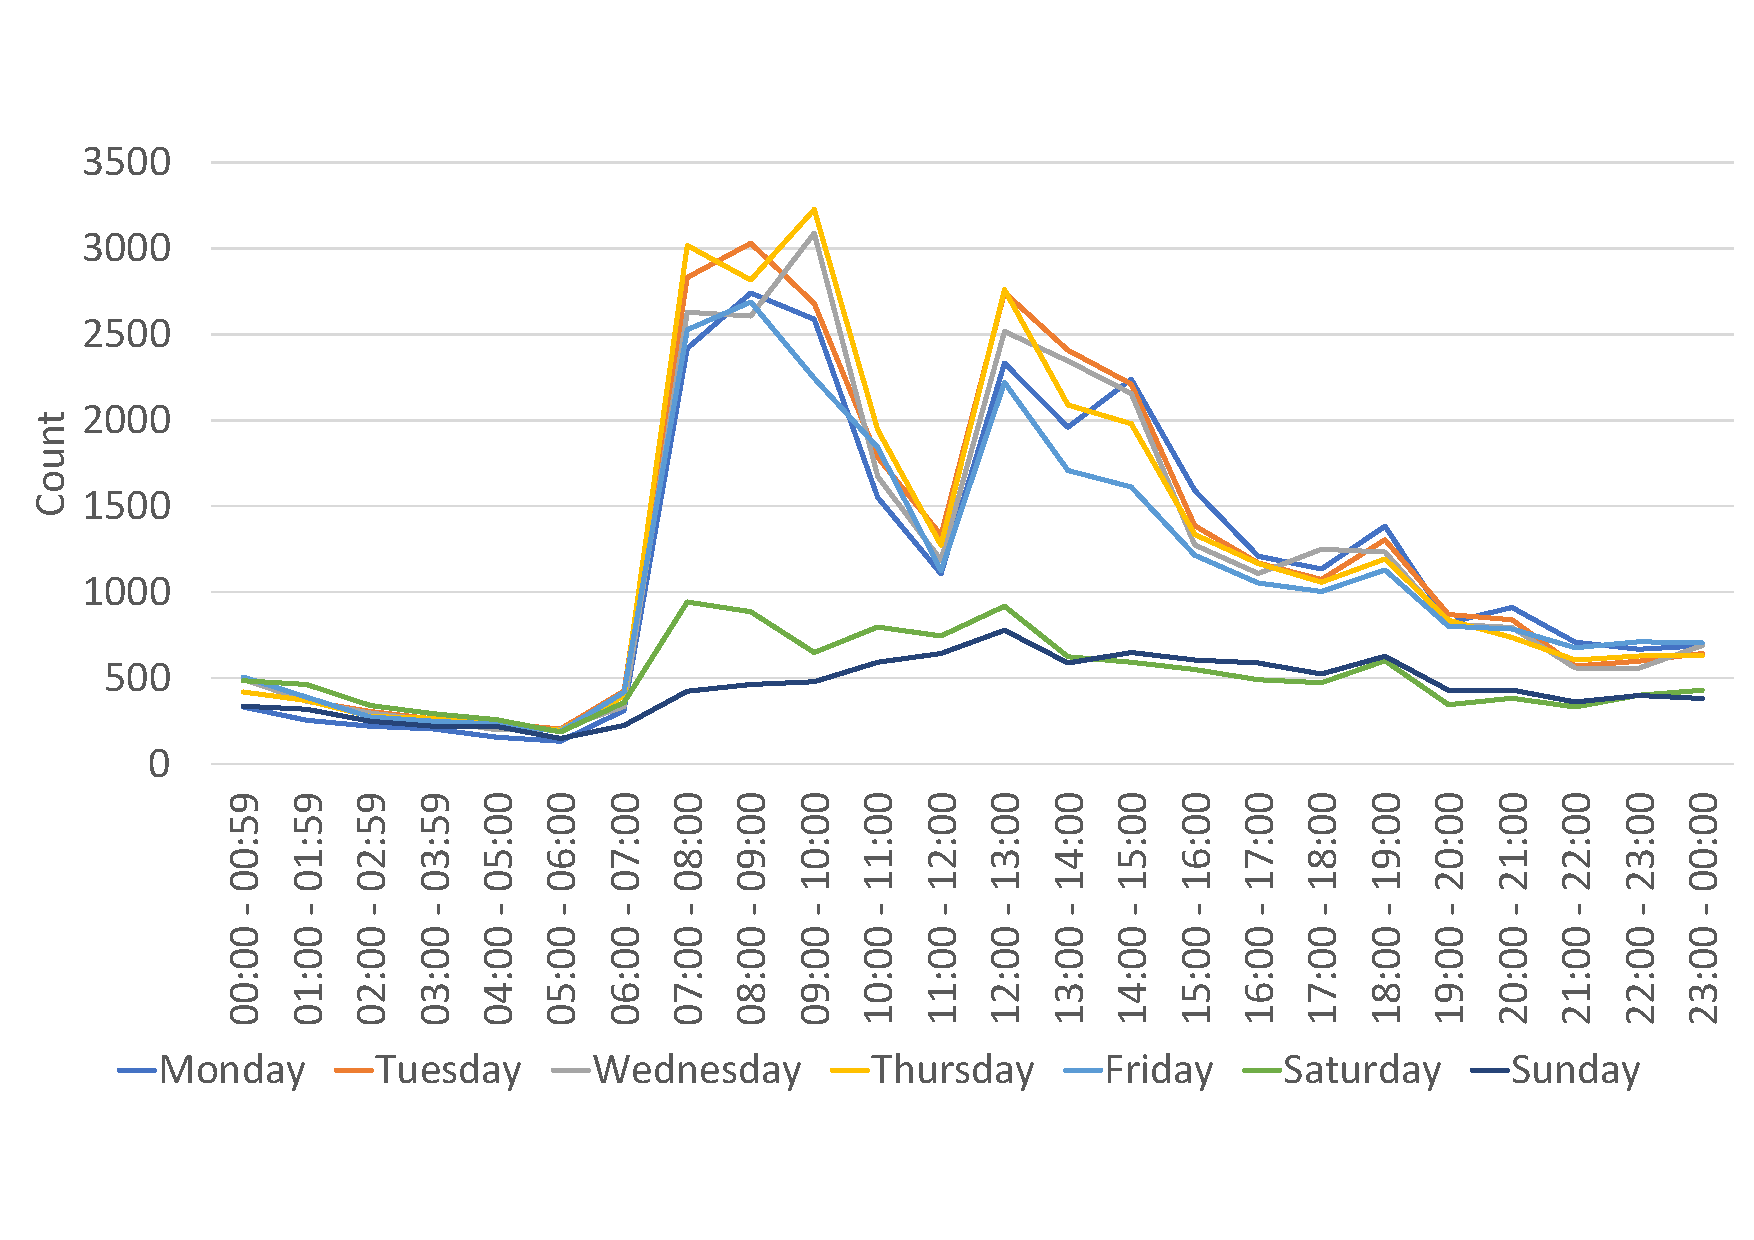
\includegraphics[width = \textwidth]{Chapter3/Figures/AdmissionTimes.pdf}
    \caption{Admissions by Hour and Day Interval}
    \label{Fig:AdmissionTimes}
\end{figure}

\subsubsection{Admission Source}\label{Sec:AdmissionSource}
The admission source of a patient determines where a patient was directly prior to admission. In total there are 25 different admission sources listed, however the top six admission sources account for 98.63\% (Table \ref{Tab:Admission Source}). If this were to be extended to include the top ten, 99.88\% of admissions would be accounted for. The top two admission sources, `Usual Place of Residence' and `Own Home' have a total count of 147,294 patients (89.21\%).
\begin{table}[h!]
    \centering
    \begin{tabular}{lcc}\toprule
    \textbf{Admission Source} & \textbf{Count} &\textbf{Proportion} \\ \midrule
    Usual Place of Residence &	99464 & 60.24\% \\
Own Home&	47830 & 28.97\%\\
Same Trust-General or young phys.disabled&	7711 &4.67\%\\
Patient transfer within the same health board/trust	&4350 &2.63\%\\
Non NHS (other then L.A.) run res.care home&	1755 &1.06\%\\
Non NHS (other than L.A.) run nursing home&	1314 &0.80\%\\
 \bottomrule
    \end{tabular}
    \caption{Top Six Admission Sources}
    \label{Tab:Admission Source}
\end{table}

\subsubsection{Admission Method}
The admission method follows a similar trend to the admission source (Section \ref{Sec:AdmissionSource}), with the majority of patients being accounted for by a few methods. There are 16 different methods listed, however the top seven account for 99.23\% of patients. `Elective - waiting list' is the most common method and is one that has been arranged in advanced. The patient has been admitted via a waiting list where at the point of being put on to the waiting list, did not know their date of admission. The period in which the patient has to wait is depending on the demand for hospital resources and facilities.

\begin{table}[H]
    \centering
    \begin{tabular}{lcc}\toprule
    \textbf{Admission Method} & \textbf{Count} &\textbf{Proportion} \\ \midrule
Elective - waiting list& 73482 & 44.50\%\\
Emergency - casualty      &	39437 &23.88\%\\
Emergency - GP          &  	28169&17.06\%\\
Other - transferred from another hospital  & 	13460&8.15\%\\
Elective - booked                  &          	5950 & 3.60\%\\
Elective - planned                &            	1696 & 1.02\%\\
Emergency - other means           &            	1658 & 1.04\%\\

 \bottomrule
    \end{tabular}
    \caption{Top Seven Admission Methods}
    \label{Tab:Admission Method}
\end{table}

\subsection{Length of stay}
The length of stay of the patient is calculated by when they are admitted to the point they have been discharged from hospital. There is a wide range of LOS's ranging from 0 to 413 days. The patients length of stay (LOS) can be modelled in two ways, in hours and in days. Firstly, by how many hours they have been admitted for was calculated using the admission and discharge date/time. The average length of stay was calculated to be 155.23 hours (6.47 days). The second method of calculating LOS, meant that if a patient was admitted overnight, and additional day was added to their LOS i.e., if admitted Monday evening and discharged Tuesday morning, their LOS was 1.

Further analysing LOS in hours, the mean was 6.47 days, whilst the 75$^{th}$ percentile was 7 days. The 90$^{th}$ percentile was 18 days increasing to 30 with the 95$^{th}$ percentile. This suggests that there are some long LOS's that are skewing the mean. 81,538 (49.38\%) of patients were discharged within 24 hours, and 114,015 (69.05\%) patients were discharged within 5 days. 5\% of patients had a LOS greater than 30 days.

Figure \ref{Fig:LOS1} displays the LOS of patients up to 15 days, which shows a high proportion of patients being discharged on day 0, i.e., were not admitted overnight. Breaking this down further by day of weeek it can be seen that these high discharges occur on days 1-5, i.e., Monday - Friday. For all days, as time passes, the number of patients with that LOS decreases. 

\begin{figure}
\centering
\begin{subfigure}{.5\textwidth}
  \centering
  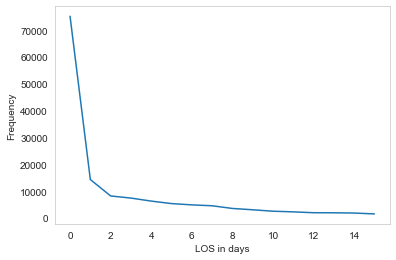
\includegraphics[width=\textwidth]{Chapter3/Figures/LOS.png}
  \caption{Total Count of LOS up to 15 Days}
  \label{Fig:LOS1}
\end{subfigure}%
\begin{subfigure}{.5\textwidth}
  \centering
  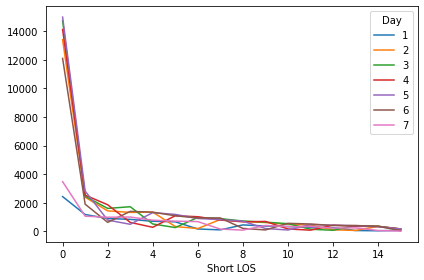
\includegraphics[width=\textwidth]{Chapter3/Figures/Short LOS.png}
  \caption{LOS by Day of Week}
  \label{Fig:LOS2}
\end{subfigure}
\caption{Length of Stay of admissions for 15 days}
\label{Fig:LOS}
\end{figure}

Depending on the day admitted, the LOS of a patient varies (Table \ref{Tab:DayLOS}). Again, patients who are admitted on a weekend have a different variation to those patients admitted during the week. The average LOS is at least an extra day longer if admitted on a weekend.

\begin{table}[h!]
    \centering
    \scalebox{1}{
    \begin{tabular}{cc}\toprule
    \textbf{Day of week} & \textbf{Average LOS} \\    \midrule
    Monday & 6.22 \\
    Tuesday & 6.12 \\
    Wednesday &6.11 \\
    Thursday &5.97 \\
    Friday &6.78  \\
    Saturday & 7.88 \\
    Sunday & 8.10  \\ \bottomrule
    \end{tabular}}
    \caption{Average LOS by Admission Day}
    \label{Tab:DayLOS}
\end{table}

Additionally, the hospital admitted to can be analysed, with Figure \ref{Fig:LOSDay} displaying that for the three most attended hospitals, mean LOS increases with age. St. Woolos Acute Hospital, shows that there is a very small increase between the means.
\begin{figure}[h!]
    \centering
    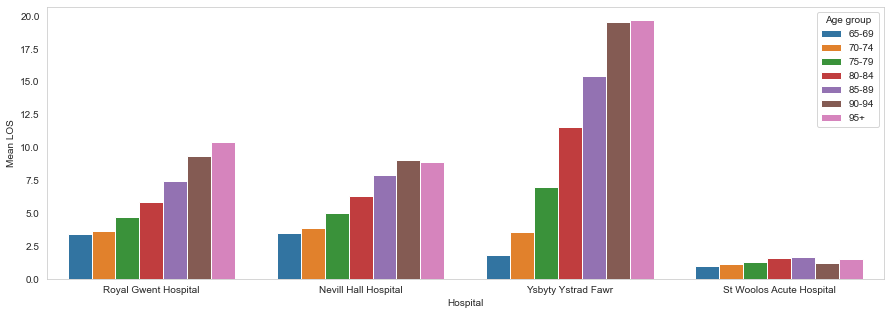
\includegraphics[width = \textwidth]{Chapter3/Figures/Mean LOS for top four hospitals in ABUHB.png}
    \caption{Mean LOS by Age Group and Hospital}
    \label{Fig:LOSDay}
\end{figure}

\subsection{Frailty Score}\label{Sec:Frailty}
Frailty score of the patients were calculated using two methods both using the ICD10 codes for the patients. In total there were 2758 different codes related to the diagnosis and reason for admission of the patient. Gilbert et al. \cite{Gilbert2018} created a hospital frailty risk score, where certain ICD10 codes were more than twice as likely to be present in a frail patient compared to a non-frail patient. This has been incorporated into our data set, so if a patient has one or more of these ICD10 codes in their stay/care spell then these scores are added together. If within a care spell, the same ICD10 code is present then the corresponding score for this code is only included once. Soong et al. \cite{Soong2015} created a list of syndromes which were more common within frailty patients. If these syndromes were present a maximum score of one was given for each hospital spell. The mean frailty score was 0.5, with a minimum value of zero and a maximum of 8.1.

When comparing the top four attended hospitals against frailty score and age group, it can be seen the mean frailty score increases with age for RGH, NHH and YYF (Figure \ref{Fig:MeanFrailty}). For YYF, the difference between the mean frailty of the youngest age group (65-69) and oldest (95+) is over 1.5.
\begin{figure}[H]
    \centering
    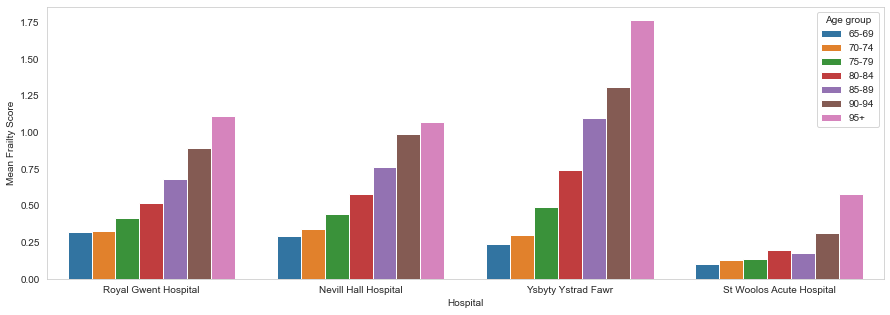
\includegraphics[width = \textwidth]{Chapter3/Figures/Mean Frailty for top four hospitals in ABUHB.png}
    \caption{Mean Frailty Score for Top 4 Attended Hospitals}
    \label{Fig:MeanFrailty}
\end{figure}

\subsection{Merging of data sets}
Once the Admission data set (Section \ref{Sec:Admission}), had been finalised with the given criteria, the Radis data set was merged to this data. This was to identify patients who had been admitted into hospital who then required a scan. For this, the Radis data set was sorted into NHS number order, with a secondary sort on dates. The NHS numbers within the Admission data set were cross referenced with the NHS numbers within the Radis data set. If there was a match, there was then a check on if the scan request date fell between the admission and discharge of the patient. If this was the case then the scan information was copied to the a results page to be placed in the same row as the admission data. As there were some patients who had multiple scans whilst in the same admission, the code ensured that all scan information for that patient was copied over, if the request date fell between the admission and discharge. This was coded within Excel VBA and the code can be found within Appendix \ref{App:ExcelVBA}.

\section{RadIS Data Set}\label{Sec:Radis}
The RadIS data set initially contained 245,287 patient records, however since we are only interested in 65 year olds and over who have been admitted, only 15,483 scan records were included (Figure \ref{Fig:Flowchart}). Table \ref{Tab:Radis} provides a detailed overview of each attribute in the data set.

%\begin{landscape}
\begin{longtable}{p{3cm}lp{5cm}ccc}
\toprule
{ \textbf{Attribute}} & {\textbf{Data type}} & {\textbf{Distinct attribute values}} & \multicolumn{2}{c}{ \textbf{Documentation}}
\tabularnewline
& &\textbf{or bins} & {at admission }&  {during stay}\tabularnewline
\midrule
\endhead

{Attendance Date} & {Nominal} & {1090 (e.g. 20170401)}&\checkmark\tabularnewline\midrule
{Attendance Time} & {Continuous} & {11417 (hh:mm:ss)} &\checkmark\tabularnewline\midrule
{Date of Birth} & {Continuous} & {7500 (e.g. 20000101)} &\checkmark \tabularnewline\midrule
{Hospital} & {Nominal} & {9 (e.g. Chepstow Community Hospital)} &\checkmark \tabularnewline\midrule
{Location Name} & {Nominal} & {74 (e.g. Medical Assessment)}&\checkmark \tabularnewline\midrule
{NHS Number} & {Nominal} & {12,299}  &\checkmark \tabularnewline\midrule
{Locality} & {Nominal} & {66 (e.g. Newport LHB, Monmouthshire LHB)} &\checkmark  \tabularnewline\midrule 
{Patient Postcode} & {Nominal} &{5484 (e.g. NP20 2UB)}  &\checkmark \tabularnewline\midrule
{Resident HB} & {Nominal} & {48 (e.g. 7A6)} &\checkmark \tabularnewline\midrule
{Request created date} & {Nominal} & {1090 (e.g. 20170401)}  & &\checkmark\tabularnewline\midrule 
{Procedure Group} & {Nominal} & {16 (e.g. R, CT)} & &\checkmark \tabularnewline\midrule 
{Exam} & {Nominal} & {293 (e.g. CT Neck and thorax)} & &\checkmark  \tabularnewline\midrule 
{Exam Code} & {Nominal} & {295 (e.g. XR Chest)} &&\checkmark  \tabularnewline\midrule
{Referring GP Practice HB} & {Nominal} & {4 (e.g. 7A5, 7A6, 7A7, X98)} &\checkmark \tabularnewline\midrule 
{Specialty Code} & {Nominal} & {37 (e.g. Gastro, Neuro)} &\checkmark\tabularnewline\midrule
\bottomrule
\caption{List of attributes within Radis data set\label{Tab:Radis}}
\end{longtable}
%\end{landscape}


Patients admitted into hospital can be given multiple scans, depending on their condition and treatment. It was calculated that there were 12,350 unique patient stays of which 9,863 patients had one scan only (Table \ref{Tab:Scan}). There were 2,487 patients who had two scans, of which 1,957 patients who only had two scans. One patient had a total of eight scans. 

\begin{table}[H]
    \centering
    \begin{tabular}{lccccccc}\toprule
    \textbf{Scan Number} & \textbf{1} & \textbf{2} & \textbf{3} & \textbf{4} & \textbf{5} & \textbf{6} & \textbf{8}   \\ \midrule
\textbf{Count} & 9863 & 1957 & 437 & 77 & 11 & 4& 1\\ \bottomrule
    \end{tabular}
    \caption{Number of Patients against Number of Scans}
    \label{Tab:Scan}
\end{table}


%\hl{Here Maybe talk about the attributes of the scan data in more detail?}\\
\\
The remainder of the scan data analysis will focus on the first scan on the patient only (12,350 patients). All scans were requested on the same day of admission, therefore the time delay between the scan being requested and the patient having the scan is due to resources. When analysing the admission day of these patients, 15.55\% are admitted over a weekend (760 on a Saturday and 1024 on a Sunday (Figure \ref{Fig:RadisDay}). Fridays are the most populous days for admissions (2,217 patients) who go on to then require a scan.

\begin{figure}[H]
    \centering
    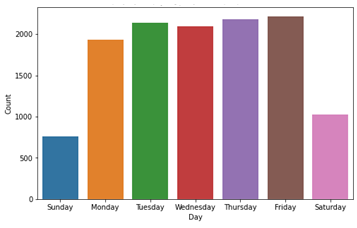
\includegraphics[width = 8cm]{Chapter3/Figures/RADIS-Day.png}
    \caption{Admission day of Scan Patients}
    \label{Fig:RadisDay}
\end{figure}

This can be further broken down into the day of the scan against the day of admission. Figure \ref{Fig:RadisDayScan} shows the day of admission of a patient, split by whether that patient had a scan on the same day of admission or at a later day. Over the weekend, only 878 patients did not have a scan on the same day as arrival. Tuesday admission had the highest quantity of patients which did not have the scan on the same day (22.67\%).

\begin{figure}[H]
    \centering
    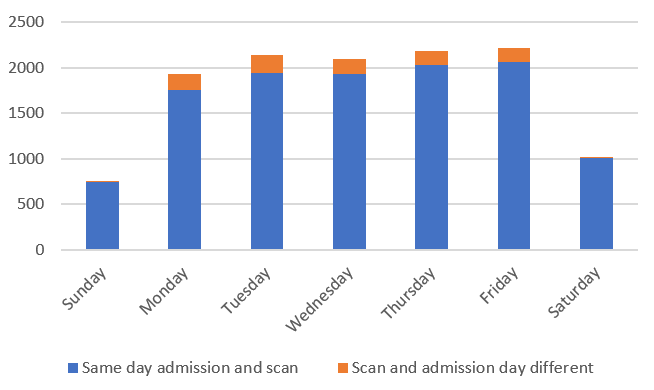
\includegraphics[width = 8cm]{Chapter3/Figures/Day against scan day.png}
    \caption{Admission day of Scan Patients Against Scan Day}
    \label{Fig:RadisDayScan}
\end{figure}

For the 878 patients who had their scan on a different day the average time it took for the patient to have a scan was 1.9 days. The longest a patient had to wait was 47 days. For this patient they spent 23 days in hospital and was then discharged to wait a further 24 days for a scan. The average length of stay for a patient who had a same day scan was 8.4 days, however this increases to 9.9 days if they did not have the scan on the same day - a difference of 37 hours. 



\begin{figure}[H]
    \centering
    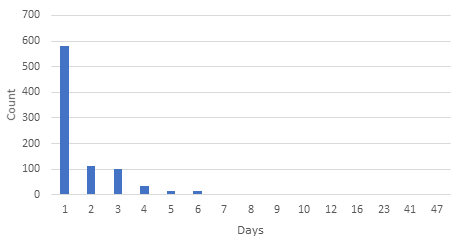
\includegraphics[width = 8cm]{Chapter3/Figures/ScanWaitTime.png}
    \caption{Admission day of Scan Patients Against Scan Day}
    \label{Fig:ScanWaitTime}
\end{figure}

This can be broken down by the day of admittance. From Figure \ref{Fig:ScanDelayDay}, it can be seen that on day three, the majority of scans is taken up by Friday admissions, i.e., these patients are waiting until Monday for their scan. Interestingly, patients who were admitted between Monday and Thursday, either had their scan before the weekend or then waited until the following week - zero patients had their scan over the weekend.

\begin{figure}[H]
    \centering
    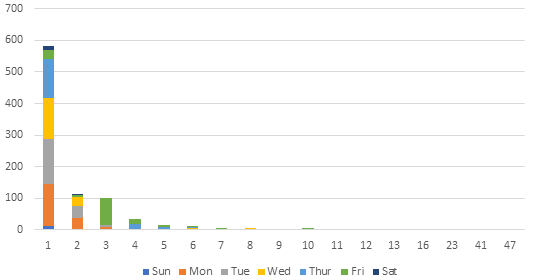
\includegraphics[width = 8cm]{Chapter3/Figures/ScanDelayByDay.png}
    \caption{Admission day of Scan Patients Against Scan Day}
    \label{Fig:ScanDelayDay}
\end{figure}

\subsection{Comparisons between scan patients and no scan patients}
A small proportion of patients require a scan whilst being admitted to hospital (7.48\%). Analysing by where the first scan took place, there were 9 different hospitals in which patients had a scan at. However, only four hospitals had attendances of over 13 patients. These four hospitals were: Royal Gwent Hospital, Nevill Hall Hospital, Ysbyty Ystrad Fawr and St Woolos Acute Hospital.

Comparing between patients who had a scan at one of the four hospitals compared to those who did not have a scan, it can be seen that for all hospitals both the average age and LOS was higher for patients who needed a scan (Table \ref{Tab:Scancomp}).
\begin{table}[H]
    \centering
\begin{tabular}{ccccc}
\toprule
\multirow{2}{*}{} & \multicolumn{2}{c}{{No Scan Patients}} & \multicolumn{2}{c}{{Scan Patients}}  \\
& {Average Age}& {Average LOS} &Average Age& {Average LOS} \\\midrule
Nevill Hall Hospital  & 77.74& 5.30 &78.33 & 8.36\\
Royal Gwent Hospital &72.24 &4.89&77.97&8.49\\
St Woolos Acute Hospital & 74.77 &1.32 &73.40 &1.71\\
Ysbyty Ystrad Fawr &75.70 &7.05&76.21&7.14\\%\midrule 
Total &77.02 & 5.02 & 77.68 &8.03\\
\bottomrule
    \end{tabular}
    \caption{Comparison of Averages between Scan and No Scan Patients}
    \label{Tab:Scancomp}
\end{table}

The top diagnoses were also different depending on if a patient required a scan, as shown within Table \ref{Tab:Scancomp2}. `Psoriasis, unspecified', `Urinary tract infection, site not specified', `Diverticular disease of large intestine without perforation or abscess', `Disorder of skin and subcutaneous tissue, unspecified' and `Pneumonia, unspecified' are the only diagnosis types to occur in the top 10 diagnosis results for both patient types. 

\begin{table}[H]
    \centering
    \begin{tabular}{cp{5.5cm}cp{5.5cm}c}\toprule
    \textbf{Ranking}& \textbf{No Scan Patients} & \textbf{Count} & \textbf{Scan Patients} & \textbf{Count}   \\ \midrule
   1 & Cataract, unspecified  & 5899& Psoriasis, unspecified&	1023 \\
2&Urinary tract infection, site not specified   &  2335&Disorder of skin and subcutaneous tissue, unspecified	&970 \\
3&Psoriasis, unspecified& 2316 &Diverticular disease of large intestine without perforation or abscess	&750\\
4&Gonarthrosis, unspecified& 2189 &Urinary tract infection, site not specified&	421 \\
5&Lobar pneumonia, unspecified   & 2150& Pneumonia, unspecified&	395\\
6&Diverticular disease of large intestine without perforation or abscess&	2082&Tendency to fall, not elsewhere classified&	348\\
7&Disorder of skin and subcutaneous tissue, unspecified&	1867 &Diaphragmatic hernia without obstruction or gangrene	&330\\
8&Follow-up examination after surgery for malignant neoplasm&1851&Benign neoplasm: Sigmoid colon	&305\\
9&Pneumonia, unspecified&	1808 &Unilateral or unspecified inguinal hernia, without obstruction or gangrene&	254\\
10&Multiple myeloma&	1651 &Acute renal failure, unspecified&	254 \\
 \bottomrule
    \end{tabular}
    \caption{Top 10 diagnosis for Scan and no Scan patients}
    \label{Tab:Scancomp2}
\end{table}


\subsection{Survival Analysis}
Survival analysis is commonly used to predict the probability of survival. This can also be applied to the probability of a patient being discharged. Within ABUHB the target is for patients to be discharged within 24 hours, otherwise they are likely to be admitted for longer lengths of time. The Kaplan-Meier survival estimate can be used to calculate the probability of discharge (Equation \ref{eq:KPSE}).

\begin{equation}\label{eq:KPSE}
    S_{t} = \frac{\text{No. of subjects in hospital at the start} - \text{No. of subjects discharged}}{\text{No. of subjects in hospital at start}}
\end{equation}
Equation \ref{eq:KPSE2} denotes the probability of admission up to day t.

\begin{equation}\label{eq:KPSE2}
    S_{t} = S_{t-1} * S_{t-2} * ... * S_{0}
\end{equation}

\begin{landscape}
\begin{table}[h!]
\centering{
\begin{tabular}{ccccccc}
\toprule
\multirow{2}{*}{Time or event (t)} & \multirow{2}{*}{No. discharged} & \multicolumn{1}{c}{No. still admitted} & \multicolumn{2}{c}{Estimated Probability} & \multicolumn{1}{c}{ Probability of still} \\ \cline{4-5}
&& at start of day& Discharged (d/n)& Still admitted 1- (d/n)& being admitted at time (T)\\ \midrule
1& 14350&89902&0.1596&0.8404& 0.8404\\             
2&8223&75552&0.1088&0.8912& 0.8404 x 0.8912 = 0.7490 \\              
3&7430&67329&0.1104&0.8896& 0.7490 x 0.8896 = 0.6663 \\    
4&6308&59899&0.1053&0.8947& 0.663 x 0.8947 = 0.5961 \\    
5&5378&53591&0.1004&0.8996& 0.5363 \\    
10&2537&32118&0.0790&0.9210& 0.4939 \\    
15&1526&21521&0.1053&0.8947&0.4419 \\    
20&995&15445&0.0644&0.9356& 0.4134\\    
25&620&11349&0.0546&0.9454& 0.3908\\
30 & 425& 8516 &0.0499&0.9501&0.3713\\\bottomrule
\end{tabular}}
\caption{Survival Analysis of all Patient Admissions {\hl{double check formatting}}}
\end{table}
\end{landscape}

The estimates obtained are explained in graph form. The graph plotted between estimated survival probabilities (Y axis) and time past entry into hospital (X axis) consists of horizontal and vertical lines. The survival curve is drawn as a step function: the proportion surviving remains unchanged between events (Figure \ref{Fig:SurvivalAnalysis1}).

\begin{figure}[H]
    \centering
    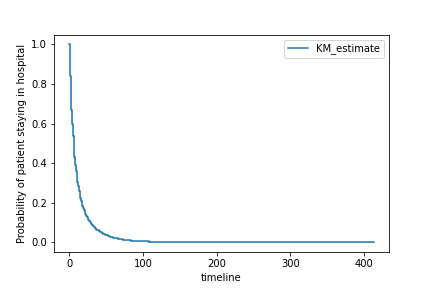
\includegraphics[width = 8cm]{Chapter3/Figures/SurvivalAnalysis.png}
    \caption{Survival Analysis of patients}
    \label{Fig:SurvivalAnalysis1}
\end{figure}
%Survival analysis on day 0

We can compare curves for two different groups of subjects. For example, compare the discharge pattern for subjects admitted to two different hospitals. We can look for gaps in these graphs in either a horizontal or vertical position. A horizontal gap means it took longer for one group to experience a certain fraction of discharges. A vertical gap means at a specific time point, one group had a greater fraction of subjects discharged.
\begin{figure}[H]
    \centering
    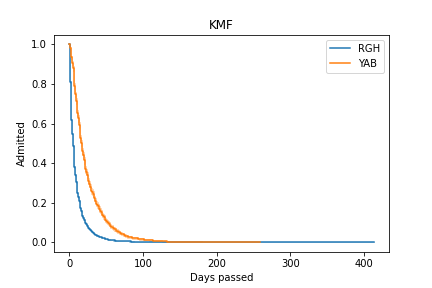
\includegraphics[width = 8cm]{Chapter3/Figures/RGH-YAB.png}
    \caption{Survival Analysis of patients who attended two difference hospitals}
    \label{Fig:SurvivalAnalysis2}
\end{figure}
Figure \ref{Fig:SurvivalAnalysis2} demonstrates the difference between an acute (RGH) and community hospital (YAB) in ABUHB. The results show that RGH patients have a higher probability of being discharged sooner when compared to YAB patients. Table \ref{Tab:SurvivalAnalysisRGHYAB} displays the difference in probabilities between the two hospitals. At day 10, there is a 40.72\% higher probability that if admitted to YAB the patient will still be admitted in hospital compared to RGH.

\begin{table}[H]
%\begin{adjustwidth}{-1.1cm}{}
\centering\scalebox{0.75}{
\begin{tabular}{cccc}
\toprule
{Time or event (t)} & RGH Probability Admitted at Time (T) &YAB Probability Admitted at Time (T)& Difference\\ \midrule
1& 0.8111&0.9840& 0.1729\\             
2 &0.7056&0.9605&0.2549\\              
3 & 0.6201&0.9356&0.3155\\    
4& 0.5492&0.9066&0.3574\\    
5 & 0.4877&0.8785&0.3908\\    
10 & 0.2770&0.6842&0.4072\\    
15 & 0.1710&0.5257&0.3547\\    
20 & 0.1133&0.4135&0.3002\\    
25& 0.0771&0.3256&0.2485\\
30& 0.0538&0.2590&0.2052\\\bottomrule
\end{tabular}}
\caption{Survival Analysis of all RGH vs YAB Patient Admissions}
\label{Tab:SurvivalAnalysisRGHYAB}
%\end{adjustwidth}
\end{table}


%The two survival curves can be compared statistically by testing the null hypothesis, i.e., there is no difference regarding discharge. The null hypothesis is statistically tested by the log-rank test, where we calculate the expected number of events in each group, i.e., E$_{1}$ and E$_{2}$ while O$_{1}$ and O$_{2}$.

%\begin{equation}
%    \text{Log-rank test statistic} = \frac{(O_{1} - E_{1})^{2}}{E_{1}} + \frac{(O_{2} - E_{2})^{2}}{E_{2}} 
%\end{equation}
%\hl{Add the code?}
% Need to check this code is working first!
\section{Data Insights}

The information from the combined data sets provides 165,118 patient records over a three year period with admissions remaining constant throughout this time. There are a higher concentration of arrivals from populous towns and cities in South East Wales, such as Caerphilly and Newport, with fewer arrivals from remote areas within the region. The higher attended hospitals tended to be the acute hospitals with 24/7 services in the region, similarly located in Caerphilly and Newport. Admissions tend to be higher during the week, with peak admissions arriving on a Tuesday. For all arrivals, there tended to be peaks in the late morning, early afternoon, and a smaller peak in the evening. The patient demographics are varied amongst all hospitals, however the length of stay within hospital varies within both age and hospital attended. The trends show that shorter LOS are more common at acute hospitals with longer LOS's at more community based hospitals. The age of the patients are fairly mixed, however the majority are aged between 65 and 85. The frailty scores of the patients provide some indication on the severity of the illness. For certain hospitals, a higher frailty score is correlated with longer lengths of stays and older age of patients. There were a small subset of admitted patients who require at least one scan within hospital.


%\section{RadIS Data Set}\label{Sec:Radis}
%\end{landscape}

\end{document}
